\section{Introduction}

% \begin{figure}[t!]
%     \centering
%     \includegraphics[width=\linewidth]{figures/pipeline/ai4science_ideal_process.pdf}
%     \caption{\textbf{AgentSLR follows a co-design process grounded in domain expert practice.} In-domain experts (epidemiologists) execute established review routines to produce expert-curated ground-truth artefacts. AI researchers consult domain experts to identify workflow bottlenecks and develop agentic routines. Resultant AI-generated artefacts are validated against ground truth and through structured assessment by the original annotators.}
%     \label{fig:placeholder}
% \end{figure}

% Wide shot:
Modern AI systems, powered by large language models (LLMs), demonstrate the ability to answer expert-level scientific questions \cite{reinGPQAGraduatelevelGoogleproof2024}, support extended reasoning tasks \cite{kwaMeasuringAIAbility2025}, interpret scientific figures \cite{robertsSciFIBenchBenchmarkingLarge2024} and generate code for research problems \cite{tianSciCodeResearchCoding2024a}. These advances suggest that LLMs might be able to automate complex, multi-stage scientific workflows that currently require substantial human expert effort \cite{wangScientificDiscoveryAge2023, zhang2025exploring, lu2024aiscientist}. Systematic literature reviews (SLRs)---comprehensive syntheses that require the retrieval, screening, extraction and analysis of up to thousands of scientific articles---represent a challenging test case \cite{zahaviHowLargeLanguage2025}. The benefits of such automation are significant, as traditional SLR workflows are resource‑intensive, taking on average 67 weeks \citep{borah2017analysis, michelson2019significant} and \$141,000 in labour to complete \citep{michelson2019significant}.

% Niche:
Empirical studies of LLM-assisted scientific evidence-based workflows, akin to SLRs, suggest that LLMs can reduce the workload of title and abstract screening \citep{oami2024performance}. However, their non-trivial false positive and false negative rates and their sensitivity to prompt choice indicate that careful agent design is preferable to end-to-end automation. Beyond screening, LLM failures relevant to scientific use have been documented previously: when summarising research articles, models often overgeneralise conclusions, risking summaries that omit scope-limiting details \citep{peters2025generalization}. These risks can compound in multi-stage agentic pipelines, where large-scale evaluations of multi-agent LLM systems report frequent orchestration and verification failures \citep{pan2025multiagent}.
% Long-context evaluations further show degraded use of information when key evidence appears mid-context, motivating retrieval-aware designs for long inputs \citep{liu2024lost}. 

\begin{figure*}[t!]
\centering
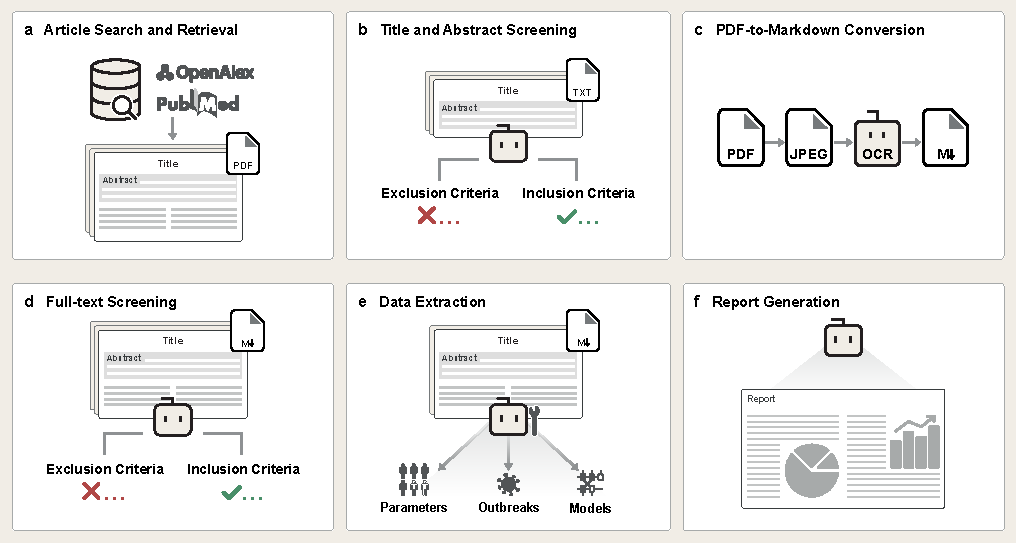
\includegraphics[width=\linewidth]{figures/flashfig_hero.pdf}
\caption{{\bf End-to-end agentic pipeline (\name) for automated systematic literature reviews}. The pipeline demonstrates a complete automation of the systematic review workflow in epidemiology, using open-source modular components. (a) \textit{Article Search and Retrieval} queries bibliographic databases with domain-specific Boolean searches and obtains PDF from open-access sources. (b) \textit{Title and Abstract Screening} applies language reasoning models to filter articles using expert-designed inclusion/exclusion criteria. (c) \textit{PDF-to-Markdown Conversion} uses an image-to-text OCR model to convert PDFs to machine-readable Markdown. (d) \textit{Full-text Screening} applies stricter filtering criteria than (b). (e) \textit{Data Extraction} employs multi-stage tool-calling with schema validation to extract structured epidemiological data (parameters, models, outbreaks). (f) \textit{Report Generation} synthesises extracted data through programmatic descriptive generation followed by iterative LRM self-refinement (writing, critique and evidence grounding). For more details see Section~\ref{sec:pipeline}.} 
\label{fig:flashfig}
\end{figure*}

% Gap:
To ground these issues in a real scientific workflow, we focus on infectious disease epidemiology as an application domain. SLRs in epidemiology often require standardised extraction of a wide range of key parameters such as the basic reproduction number, serial interval, and case-fatality ratio across diverse study designs and data representations---a task made more challenging by substantial heterogeneity in methodologies and reporting structures \citep{he2020estimation,WARD2026100882}.  We therefore select epidemiology to establish the technical feasibility of automating evidence synthesis in a specialised scientific domain. 

\vspace{1em}

% Contributions:
Our contributions are summarised as follows:
\begin{itemize}

\item We introduce \textbf{\name{}}, a fully \textit{open-source, end-to-end agentic pipeline} that uses language reasoning models (LRMs) to automate real-world systematic reviews, including article retrieval, screening, tool-based data extraction, and living systematic review generation. 

% \footnote{Code available in Supplementary Materials.}

\item We apply \name{} to epidemiology, evaluating against expert ground truth data from SLRs on WHO-designated priority pathogens. 
We demonstrate that agentic LRM systems can achieve comparable outputs to humans while processing articles $58$ times faster.

\item We validate \name{}'s extracted outputs with manual annotation by human expert epidemiologists. Annotators judge extractions to be largely accurate ($79.8\%$ average) and suggest the system would play a useful collaborative role in their review process.

\item We conduct model ablations across five frontier reasoning models (\texttt{gpt-oss-120b, GPT-5.2, Kimi-K2.5, GLM-4.7, DeepSeek-V3.2}), 
analysing the performance-to-cost trade-off across pipeline stages and identifying where model choice most impacts systematic review automation.
\end{itemize}


